\documentclass[convert]{standalone}

\usepackage{tikz}
\usepackage{graphicx}
\pagestyle{empty}

% INT_AY22_L25-Fig03_Crossed_wires.png

\begin{document}
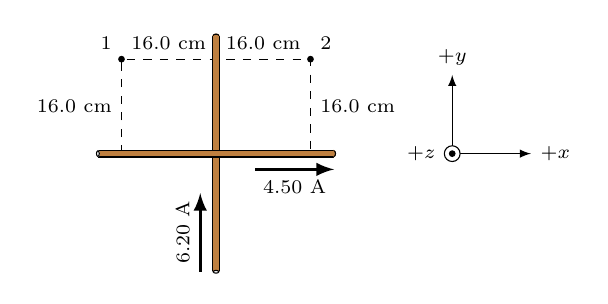
\begin{tikzpicture}[> = latex, font = \scriptsize]

	% Definition
	
	\def\L{1.2}		% Position of marked points
	
	% Marked points + distance markers
	
	\draw [fill = black] (\L, \L) circle (1 pt) node [above right] {2};
	\draw [fill = black] (-\L, \L) circle (1 pt) node [above left] {1};
	
	\draw [dashed] (-\L, 0) -- node [midway, left] {16.0 cm} (-\L, \L) -- node [midway, above] {16.0 cm} (0, \L)
		-- node [midway, above] {16.0 cm} (\L, \L) -- node [midway, right] {16.0 cm} (\L, 0);
	
	% Vertical current wire with direction
	
	\draw [double = brown, double distance = 2 pt] (0, -1.5) -- (0, 1.5);
	\filldraw [brown] (1 pt, 1.5) arc (0 : 180 : 1 pt and 0.5 pt) -- cycle;
	\filldraw [white] (1 pt, -1.5) arc (360 : 180 : 1 pt and 0.5 pt) -- cycle;
	\draw (1 pt, 1.5 cm) arc (0 : 180 : 1 pt and 0.5 pt);
	\draw (0, -1.5) ellipse (1 pt and 0.5 pt);
	
	\draw [->, very thick] (-0.2, -1.5) -- node [midway, above, rotate = 90] {6.20 A} (-0.2, -0.5);
	
	% Horizontal current wire with direction
	
	\draw [double = brown, double distance = 2 pt] (-1.5, 0) -- (1.5, 0);
	\filldraw [brown] (1.5, 1 pt) arc (90 : -90 : 0.5 pt and 1 pt) -- cycle;
	\filldraw [white] (-1.5, 1 pt) arc (90 : -90 : 0.5 pt and 1 pt) -- cycle;
	\draw (1.5, 1 pt) arc (90 : -90 : 0.5 pt and 1 pt);
	\draw (-1.5, 0) ellipse (0.5 pt and 1 pt);
	
	\draw [->, very thick] (0.5, -0.2) -- node [midway, below] {4.50 A} (1.5, -0.2);
	
	% Coordinate axes
	
	\draw [<->] (3, 1) node [above] {$+y$} -- (3, 0) -- (4, 0) node [right] {$+x$};
	
	\draw [fill = white] (3, 0) circle (0.1) node [left = 0.25 em] {$+z$};
	\filldraw (3, 0) circle (1 pt);

\end{tikzpicture}
\end{document}